%----------------------------------------------------------------------------------------
%                   Galway-Mayo Institute of Technology (GMIT)
%                Department of Computer Science and Applied Physics
%
%                      *** Latex template for dissertations ***
%----------------------------------------------------------------------------------------

\documentclass[oneside]{book}

\usepackage{graphicx} % Required for the inclusion of images
\usepackage[numbers]{natbib} % Required to change bibliography style to APA
\usepackage{amsmath} % Required for some math elements 
\usepackage{makecell}
\usepackage{eurosym}
\usepackage{tabularx}
\usepackage{pbox}
\usepackage{listings}

\setlength\parindent{0pt} % Removes all indentation from paragraphs

% \usepackage{geometry}
% \geometry{margin=.5in}


\newcommand*{\customTitle}{\begingroup % Create the command for including the title page in the document
\centering % Center all text
\vspace*{\baselineskip} % White space at the top of the page

\rule{\textwidth}{1.6pt}\vspace*{-\baselineskip}\vspace*{2pt} % Thick horizontal line
\rule{\textwidth}{0.4pt}\\[\baselineskip] % Thin horizontal line

%----------------------------------------------------------------------------------------
%	1) Change Dissertation Title
%----------------------------------------------------------------------------------------
{\Large A Job Portal For Software Developers}\\[0.2\baselineskip] % Title
%----------------------------------------------------------------------------------------


\rule{\textwidth}{0.4pt}\vspace*{-\baselineskip}\vspace{3.2pt} % Thin horizontal line
\rule{\textwidth}{1.6pt}\\[\baselineskip] % Thick horizontal line
\scshape % Small caps \\[\baselineskip] % Tagline(s) or further description
\Large \textbf{Final Year Project}\\
\textbf{B.Sc.(Hons) in Software Development}\par % Location and year
\normalsize
\vspace*{2\baselineskip} % Whitespace between location/year and editors


%----------------------------------------------------------------------------------------
%	2) Change Student Name(s)
%----------------------------------------------------------------------------------------
{by \\ Neil Kyne \par} % Editor list
%----------------------------------------------------------------------------------------


\vspace*{2\baselineskip} % Whitespace between location/year and editors
\vfill % Whitespace between editor names and publisher logo
{\scshape \today} \\[0.3\baselineskip] % Year published
%----------------------------------------------------------------------------------------


%----------------------------------------------------------------------------------------
%	3) Change Supervisor
%----------------------------------------------------------------------------------------

{\textbf{Advised by Dr. John French}}\par % Supervisor

{Department of Computer Science and Applied Physics Galway-Mayo Institute of Technology (GMIT)}\par % Department
%----------------------------------------------------------------------------------------


\endgroup}
\begin{document}
\pagenumbering{gobble}
\begin{figure}
\begin{center}

\includegraphics[width=8cm,height=3.3cm,keepaspectratio]{gmit-logo} % Include the image placeholder.png
\end{center}
\end{figure}
\customTitle % This command includes the title page
\tableofcontents
\listoffigures
\pagenumbering{arabic} 

\chapter*{Abstract}
This final year project was inspired by my desire to develop a practical web application. A project that could give me a sense of what it would be like to work on a production ready application in this industry today. I chose to make it a job portal aimed at developers simply because I felt it would further engross me into this industry further.

The application uses React as its primary technology with an API built using Spring Boot. All of the job data is hosted on MongoDB Atlas. It uses JWT for user authentication and is fully deployed on Heroku.

The application itself contains many features such as the ability to login and logout, perform CRUD functionalities on jobs as well as custom searches. The main goal in developing the front-end was to make it as 'Reactful' as possible, minimising repeat code by using as many components as possible while developing the back-end focused more on ensuring the API was RESTful.

The following document details my development journey throughout my final year, from initial research into technologies I was interested in using to problems faced during development.


%----------------------------------------------------------------------------------------
%	4) Change Chapters
%      Write each chapter in a separate TEX file and include here
%----------------------------------------------------------------------------------------

\chapter{Introduction}
The following document is a dissertation for my final year project in which I hope to achieve a B.Sc. (Hons.) in Software Development. This project was undertaken by just myself and all work shown is my own.

From the beginning of the year I knew I wanted to make a practical web application, a website that could actually be useful to people and would also provide me with a suitable challenge and rewarding, worthwhile learning outcomes. Much research went into what kind of project I would do and what technologies I would use to do it which will be discussed further on in the document.

The finished project however is a job site for software developers. I opted to use mainly React, a Javascript library for the front-end along with some accompanying frameworks and used Spring Boot for the back-end as well as MongoDB for the database.

\section{Early Research}
Initially the project was going to take a much different shape in my mind. I had planned on it being more of a general purpose 'odd-job' type app where users could post or accept listings advertising a certain amount of pay for menial jobs such as mowing a lawn or cleaning up around a house etc.

As the idea grew in my head I realised I would prefer it to be specific to my field of study. I decided my project would be a job site specifically for software developers. This way I could incorporate OAuthentification into the website with developers logging in via their LinkedIn or even Github accounts. This would tie in nicely to the general theme and purpose of the website. OAuth doesn't share password data but instead uses authorization tokens to prove an identity between consumers and service providers. OAuth is an authentication protocol that allows you to approve one application interacting with another on your behalf without giving away your password \cite{OAuth}.

\subsection{MEAN Stack}
I had initially planned on developing the project using the MEAN stack. The MEAN stack (MongoDB, Express.js, AngularJS and Node.js) is a free and open-source JavaScript software stack for building dynamic web sites and web applications \cite{mean}. Because all components of the MEAN stack support programs that are written in JavaScript, MEAN applications can be written in one language for both server-side and client-side execution environments. However, after discussing it with my supervisor, I learned that this might not have appeared challenging enough to some as it had already been covered in the previous year. A big part of the applied project is to showcase self learning and the ability to understand foreign concepts that haven't been explicitly taught in class. Although I joined this year after 2 years out of college I agreed it would be better if I tried to show technologies not already covered on the curriculum and weren't seen before among this group of students.

\subsection{MERN Stack}
After deciding against the MEAN stack, I looked into the MERN stack (MongoDB, Express, React, and Node. js), again however, there wasn't really enough variation in language and I would have been making a glorified JavaScript application.

\subsection{Dropwizard \& Spring Boot}
I decided I was trying too hard to conform to a predefined 'stack' and realised I didn't have to choose a set of technologies that work well together just because they form a nice acronym. I wanted to have a back-end built in a language other than JavaScript and for developing RESTful web services you don't need to look much farther than DropWizard or Spring Boot.

\subsubsection{Dropwizard}
Dropwizard is a Java framework for developing web services in Java. Dropwizard makes use of multiple different packages such as \textbf{Jetty, Jersey and Jackson} that let you deploy a micro-service with relative ease\cite{dropwizard}. On top of that, we were actually using Dropwizard in our first semester for the module 'Distributed Systems' so I would have had the added help of knowledge gained from these assignments.

\subsubsection{Spring Boot}
The other technology I looked into was Spring Boot. Like Dropwizard, Boot makes it all too easy to get a Java web application up and running in mere minutes. Spring Boot is a Spring framework module which provides Rapid Application Development (RAD) feature to the Spring framework. It is highly dependent on the starter templates feature which is very powerful and works flawlessly \cite{boot:howto}.

I did a lot of research into these two technologies and found that I was only one of a great many developers unsure about which one to go for. There are countless articles and websites online going into great details comparing the two frameworks and I found it quite easy to get bogged down by an overload of information on the two (Figure ~\ref{drop_label}). In the end I opted for Spring Boot, I found examples of how well it interacts with MongoDB and decided that would be very useful in my application. I don't think development of the API would have suffered at all had I gone for Dropwizard, they're both clearly two very popular technologies for Java web development.

\begin{figure}[h]
    \centering
    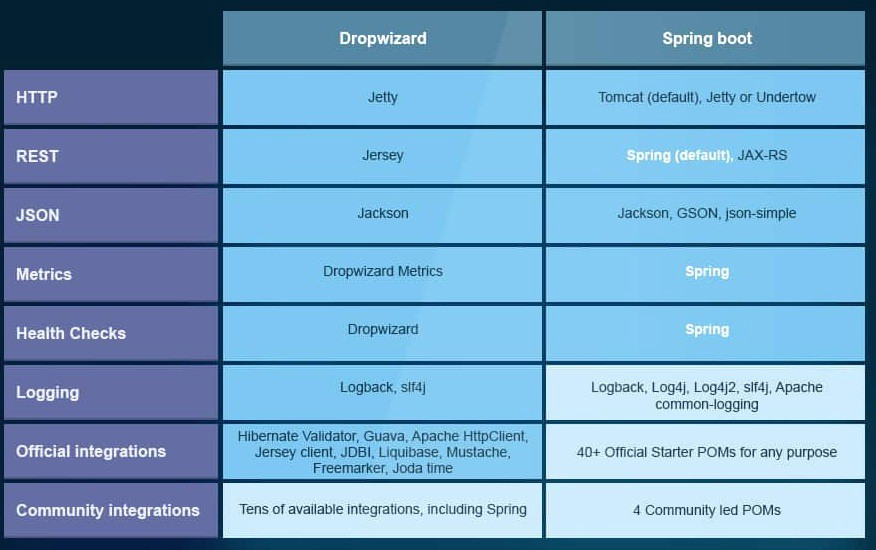
\includegraphics[scale=0.3]{Images/dropwizard.jpeg} 
    \label{drop_label}
    \caption{Comparison of 3rd party libraries}
\end{figure}

\section{What the Project Brings}
The premise of the project as touched on above, was to bring a small number of technologies together, and have them working efficiently and effectively with a clear reason for their use. As it was just myself in the group, I was generally happy for the scope to be a bit smaller as long as the project itself was an effective program functioning well across different levels in the stack.

The 3 main technologies effectively offer everything a web application would need to be deployed and used by an actual user.

\section{Scope}
As mentioned earlier, I developed the project by myself. Taking this into consideration I felt that a full stack application, hosted online was suitably challenging. The project's architecture consists of three unique tiers all communicating in a stack to form the web application. The three parts are as follows: 

\subsection{Database/Back-End Tier}
I used MongoDB for my database technology. MongoDB is a NoSQL database, it is document oriented and it stores data in collections instead of tables \cite{parker2013comparing}. The main use of the database is to store my job objects. The users of my application can perform basic CRUD functionality on the jobs stored in the database. My MongoDB database is hosted on a cloud service called MongoDB Atlas. This is done so that when they application is deployed online via Heroku, the data is available at all times.

\subsection{Server Side/Middle Tier}
For my 'middle' tier I used Spring Boot. Spring Boot is a fantastic variation of Spring that allows for quick painless development of a web application with almost no configuration. The RESTful API is contained in my Spring server and connects the React application to the Mongo database containing the job objects to be manipulated. The REST API is hosted as its own application on Heroku and communicates with the React application to perform requests.

A deciding factor in choosing Spring boot as my server side technology was it's very powerful MongoDB connector. All you need to do is simply extend the 'MongoRepository' class from a repository interface which contains plenty of generic methods already. Impressively, you do not need to manually implement these queries yourself, instead you can use Spring Boot's repository naming conventions, and the 'MongoRepository' will intelligently construct the queries at run-time \cite{marchioni2015mongodb}.

\subsection{Front-End Tier}
For the front end of my web application I decided to use React. React is a Javascript library for building UI's. However, as it is only concerned with rendering data to the DOM. React requires  additional libraries for state management, sending HTTP requests and routing such as React Router and Axios \cite{wiki:xxx}. I use multiple Javascript libraries in my application to compliment React such and will examine them later in the document.

I performed testing on the front-end application using two testing frameworks, 'Jest' and 'React-Testing-Library'.

\section{Objectives}
Like the vast majority of students in my year, my primary objective in developing this application was to learn a new set of skills and to become familiar with a new set of technologies. It was also a great opportunity to develop and improve my project management skills as it demands attention over an extended period of time. I believe by choosing technologies I have had no substantial previous experience with I definitely accomplished this objective. I set the following goals for my project from the very beginning of the year:

\begin{itemize}
    \item I wanted my application to have a number of moving parts and to be a real 'Full Stack Application'. I felt a 3 tier system would go a long way towards showing me how a production ready application might actually look in the working world. When developing across different levels you learn a lot about how each level of the stack works, how they communicate with each other, what works well together and what doesn't.
    \item As I have a big interest in web development in particular, I specifically wanted to become very familiar with React. According to Stack Overflow's 2019 survey, more developers say they use React.js than Angular, a switch from last year \cite{Stack}. It ranked second overall behind JQuery.
    \item Adding to what I said earlier about getting a taste for what a real world application might look, I felt it was very important to have genuine authentication. I initially wanted OAuthentication but opted instead for JSON Web Tokens or failing that, basic authentication.
    \item I wanted users to be able to perform the basic CRUD functionalities with jobs.
    \item I wanted the application to be deployed on Heroku.

\end{itemize}

\section{Documentation}
This document will give a detailed description of my research, planning, reasoning and thought process throughout the development of my application. It is split up into six chapters. Each detailing a different aspect of the work put into the application itself. They are: 

    \subsubsection{Introduction}
    The current chapter, the introduction, has covered what my aims for the project were early on. What research I did before choosing to develop using the technologies I did and also my objectives for the project before beginning development.
    
    \subsubsection{Methodology}
    This chapter will go over how I went about the development of my project at a more detailed level. It will cover how often I met with my supervisor and how often I dedicated each week to the project. It will essentially cover how I went about developing and planning the entire project, which project methodology was used and if I felt it was at the right level. 
    
    \subsubsection{Technology Review}
    This chapter will documents the outcome of my research into the technologies I used and how I used them to achieve my objectives. Every technology used in the development of the application will be described here, covering what they do in general and what they offer to my application specifically.
    
    \subsubsection{System Design}
    This section will describe the architecture of the application. It will cover how each tier of the application communicate together to form the complete project. It will contain diagrams and screenshots to help visualise the structure and architecture of the application.
    
    \subsubsection{System Evaluation}
    In this chapter I will do a full evaluation of the application as a whole. I will compare the final outcome of the application with the objectives I initially outlined in the Introduction chapter. I will also outline any limitations or difficulties I found in the project be it through technologies used or through my own decisions and mistakes. I will also suggest improvements I believe could be made on the application.
    
    \subsubsection{Conclusion}
    The conclusion will be a summary of the entire finished project. It will discuss my initial goals for the project and how well I managed to achieve them. I will cover what I feel I learned throughout the development of the project and the writing of the dissertation. It will also outline any regrets I have with the project be they from using the wrong technologies or other matters. Overall I hope it will provide a final piece of insight on my experience with the project and hopefully wrap up the documentation.
\chapter{Methodology}
\section{Initial Planning and Research}
When I first set out beginning this project I wanted to make sure I gave the planning phase enough attention. Often times in the past for previous college projects I found myself jumping straight into coding without having properly thought out and planned what I actually needed to do and in what order. This can often times lead to running into obstacles further down the line in the project that become harder and harder to revert or fix the longer they are left.

I knew I wanted to use a JavaScript framework for the front end design. As I had initially planned on using the MEAN stack for the project I brought this up with my supervisor who informed me that this stack had been covered in some degree in the previous year, therefore it might seem as if I am not challenging myself enough with a new technology. Of course, I wasn't in this year and had no prior learning with it but opted to leave it nonetheless.

After meeting my supervisor and swapping ideas I decided to do some further research into popular technologies for designing web applications and landed on React for the front end and MongoDB for the database tier. My supervisor recommended I look into Spring Boot or Dropwizard for the back-end side of things and from there I had a decent amount of material and technologies to familiarise myself with before the actual development of the application could begin.

Although testing wasn't very high on my list, as is the case for many student projects, I knew I would need to at least 'dip my toe' into it. It was important for me to gain exposure to every facet of developing a full stack application. Research into testing React applications very quickly led me to 'Jest' and 'React Testing Library' which I will cover in further detail later.

\section{Project Planning Tools and Project  Meetings}
As I did not form a group with any other students I simply set aside two hours every week for my own individual project meetings. I usually did this the day before meeting with my supervisor in order for things to be fresh in my mind with which to discuss. Of course as time goes on and depending on other project deadlines, I often went well over two hours a week and occasionally wen under this. I tried to always do something however. As I touched on before, I really didn't want to rush into coding before I had a decent idea of what I wanted to do and in what order I needed to do it. My supervisor was very helpful in this respect and used to set out weekly objectives for me to have completed before our next weekly meeting.

As far as project planning tools, I initially used Trello. Trello is a project managing software that helps to visualise projects as well as organise workloads into different cards \cite{wiki:trello}. Initially, I used Trello quite a lot for planning and research as well as making sure I set objectives and deadlines for such research (Figure ~\ref{trello_label}). As the weeks went on however I found myself using it less and less and instead, just noting what goals I wanted to achieve in a diary instead. I did this because one of Trello's main features is it's team feature which grants multiple people access to a board, as I was the only person in my project group I didn't really need to worry about the planning being online and available to team members.

\begin{figure}
        \centering
        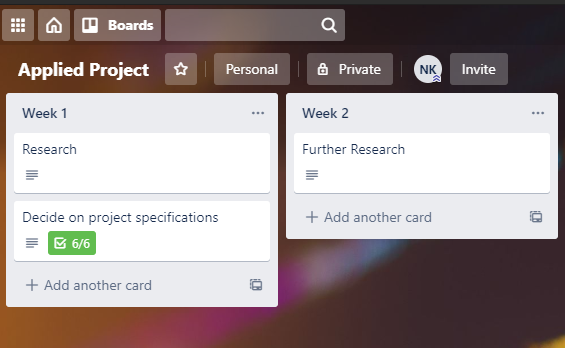
\includegraphics[scale=0.6]{Images/Trello.png} 
        \label{trello_label}
        \caption{My Trello Board}
\end{figure}

\section{Github as a Development Tool}
As with all projects I undertake, I used Git for version controlling the application as well as backing up the application. Looking back, I feel I didn't utilise Github as well as I would have liked. Github offers a lot of functionality such as the issue tracker or the wiki. I largely only used Git for backing up my project and always having the source code accessible from any device.

If I was to start the development of this project again I would definitely have used the issue tracker as often as possible to show the problems I faced with development as well as how I overcame them. I began using the issue tracker very late in the project and I only managed a small handful of entries.Not using it throughout is a  big regret I have, since I 've started using it I've found it's a great way to showcase your thinking at each stage of a problem. I also would've used branches to always keep a clean working copy of my application available that I could revert to at any time. Git is a very important tool to software development and I feel I might have used this opportunity better to showcase my understanding of it more.

The wiki is another powerful feature I might have used. The wiki provide a place in your repository to lay out the road-map of your project, show the current status, and document software better. I instead opted to simply keep a Word diary on my local machine, that I made entries to whenever I worked on the project. I believe documenting your thinking during development is very important.

\chapter{Technology Review}
% Boot - spring security, mongo, react - react router, axios, formik, bootstrap, heroku, jwt, postman
\paragraph{In this section I'll examine the different technologies that were used in the application. I'll explain why I chose to implement each one specifically and whether or not I feel they were the right choice. As well as the major technologies used I'll touch on frameworks or libraries I feel are relevant to mention for the corresponding technology. The core technologies used that I will scrutinize the most in this section are; Spring Boot, React, MongoDB and Heroku.}

\section{MongoDB}
\paragraph{MongoDB is a NoSQL document oriented database program. A MongoDB database can contain multiple collections, each record in a collection is document. Documents are a structure composed of file and value pairs, similar to JSON objects or other mapping data types \cite{Mongo:doc}. The table below (Figure ~\ref{mongo2_label}) illustrates some differences between a MongoDB database and a relational database.}
\paragraph{Not only Sequential Query Language (NoSQL) is a database type that provides a mechanism for storage and retrieval of data which is modelled by means other than the tabular relations used in relational databases, in the case of MongoDB, it is document based. NoSQL databases are a favored solution for 'Big Data' storage as they incorporate a schema-less data model \cite{wiki:nosql}. 'Schema-less' means the database doesn't have fixed data structure. A NoSQL database provides increased scalability and flexibility compared to relational databases.}
\begin{figure}[h]
    \centering
    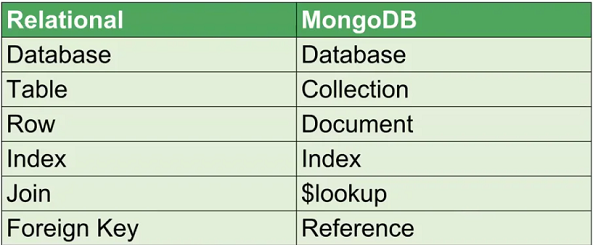
\includegraphics[scale=0.4]{Images/mongo2.png} 
    \label{mongo2_label}
    \caption{MongoDB vs relational DB}
\end{figure}

\subsection{MongoDB Atlas}
\paragraph{MongoDB Atlas is a cloud based system developed by MongoDB. Atlas provides an easy way to host and manage your data in the cloud with the service provider of your choice, for this application, I used Amazon Web Services (AWS).}
\paragraph{Atlas uses clusters to manage the data in a MongoDB project. Clusters are simply Atlas-managed MongoDB deployments and can be either a replica-set or a sharded cluster \cite{Mongo:clusters}. (Figure ~\ref{mongo3_label}) shows my atlas project is a replica set with three nodes}
\begin{figure}[h]
    \centering
    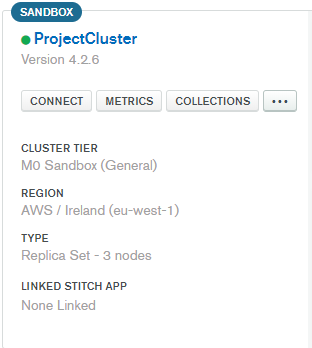
\includegraphics[scale=0.4]{Images/mongo3.png} 
    \label{mongo3_label}
    \caption{My MongoDB Project Cluster}
\end{figure}
\paragraph{A replica-set means there are multiple instances (in my case three) of MongoDB which each mirror all the data of the other. A replica-set consists of one primary node (master) and one or more secondary nodes (slaves). Read-operations can be served by any slave, but write-operations always take place on the master of the replica-set and are then propagated to the slaves. Replica-sets offer fault-tolerance as when one of the members of the replica-set goes down, the others take over. When the master goes down, the slaves will elect a new master.}
\newpage
\subsubsection{Atlas In My Application}
\paragraph{To connect my Spring Boot application to my MongoDB cluster I simply had to configure it's connection address in the 'application.properties' file (Figure ~\ref{mongo5_label}). }
\begin{figure}[ht]
    \centering
    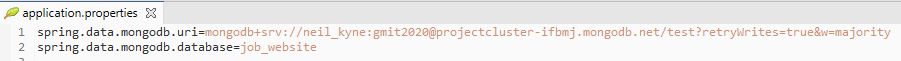
\includegraphics[scale=0.515]{Images/mongo5.png} 
    \label{mongo5_label}
    \caption{Connecting to My MongoDB Cluster}
\end{figure}
\paragraph{After providing the connection details above, our database, collection and all of the documents associated with that collection can be viewed on the MongoDB Atlas project page (Figure ~\ref{mongo1_label}).}
\begin{figure}[ht]
    \centering
    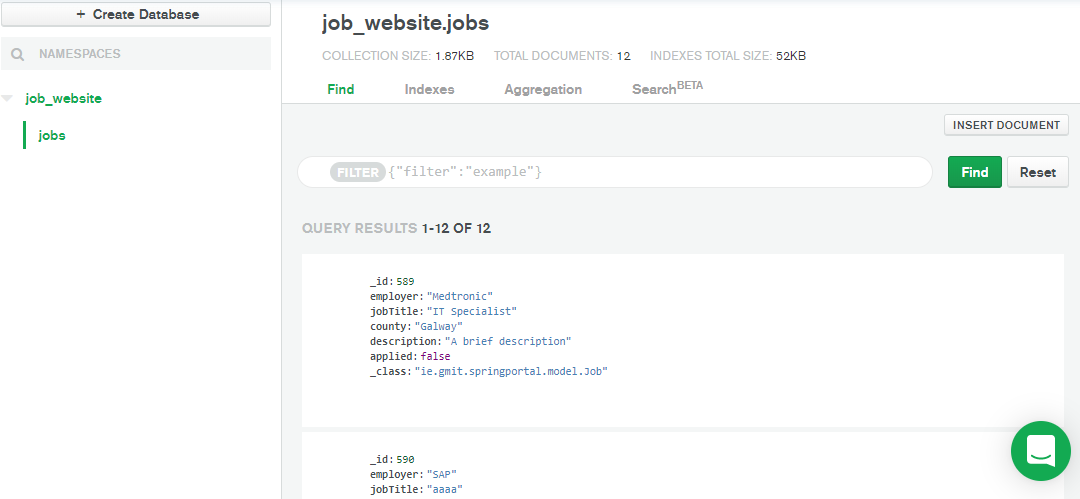
\includegraphics[scale=0.4]{Images/mongo1.png} 
    \label{mongo1_label}
    \caption{My MongoDB Database}
\end{figure}

\section{Spring Boot}
\paragraph{To properly understand Spring Boot we must first briefly summarize its foundation framework, Spring. Spring is one of the most popular Java Enterprise Edition (EE) Frameworks for building  web services. For the Java platform, the Spring framework provides an elaborate programming and configuration model. It can be used at any kind of deployment platform as unlike other frameworks, Spring focuses on several areas of an application and provides a wide range of features. However, in recent years, due to added functionalities, the Spring framework has become increasingly complex. It requires going through a lengthy procedure in order to start a new Spring project. To avoid starting from scratch and save time, Spring Boot has been introduced. This uses the Spring framework as a foundation \cite{DZone:Spring}.}
\paragraph{Spring Boot allows developers to create stand-alone, production-grade Spring based Applications that you can "just run".
It take an opinionated view of the Spring platform and third-party libraries so you can get started with minimum fuss. Most Spring Boot applications need minimal Spring configuration \cite{Spring:SpringBoot}.}
\subsection{Creating Spring Boot Application}
\paragraph{I chose to 'Bootstrap' my application with the 'Spring Initializr' provided on the official Spring website (Figure ~\ref{spring1_label}). This is a very handy tool that lets you pre-configure project settings such as dependencies, languages or project type (Maven) and get setup and ready to code within minutes.}
\begin{figure}[ht]
    \centering
    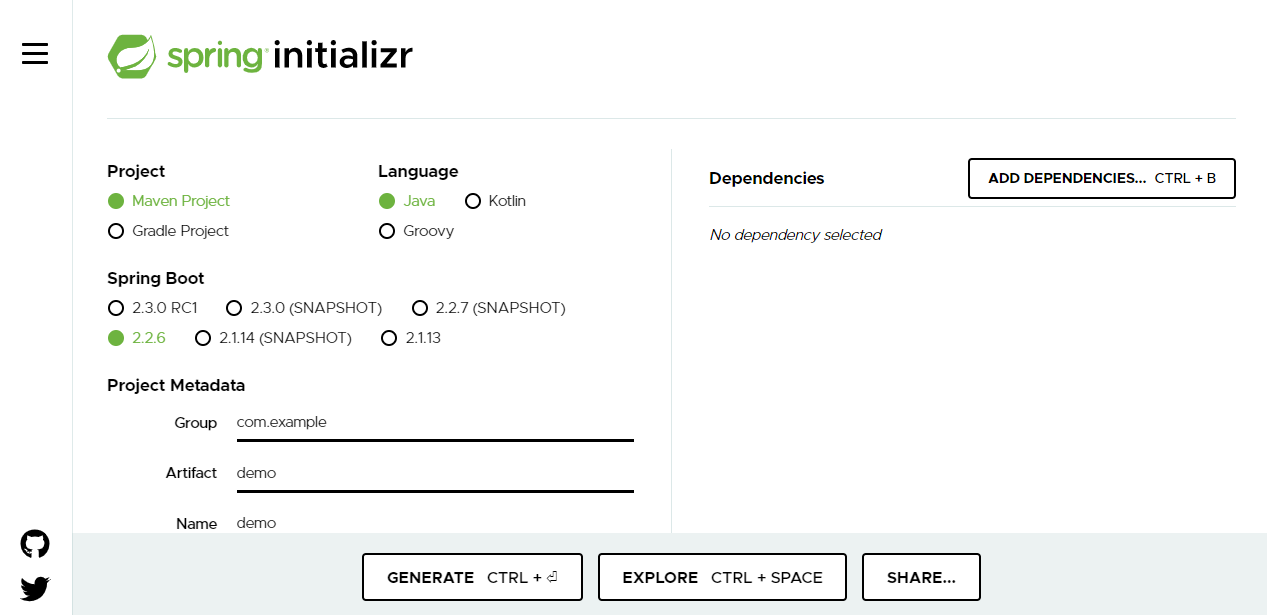
\includegraphics[scale=0.35]{Images/spring1.png} 
    \label{spring1_label}
    \caption{Spring Initializr Setup Page}
\end{figure}
\paragraph{Once I generated the Spring Boot project from the 'Initializr' I simply needed to import that package to Eclipse as a Maven project. As we can see in (Figure ~\ref{spring2_label}) all of the dependencies chosen in the Initializr have been added to the 'pom.xml' file.}
\begin{figure}[ht]
    \centering
    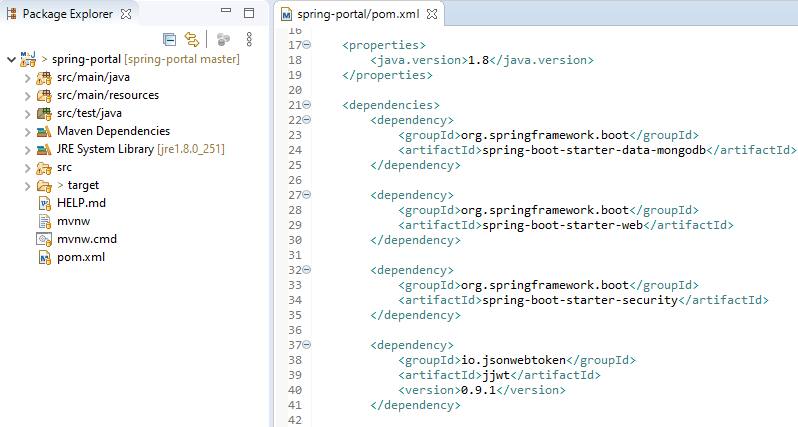
\includegraphics[scale=0.33]{Images/spring2.png} 
    \label{spring2_label}
    \caption{Spring Initializr Setup Page}
\end{figure}

\section{Heroku}
\paragraph{I mentioned earlier in the document I wanted my project to mimic what it would be like to develop a real website. Of course, my application can hardly hold a light to a user ready website we could find on the web at this moment, however, I did want it to be deployed in order to understand what is required to deploy a large application with multiple different technologies and tiers working together.}
\paragraph{With this in mind, I decided to use Heroku as I had some experience with it from the module 'Software Engineering' already this semester.
Heroku is a container-based cloud Platform as a Service (PaaS). Developers use Heroku to deploy, manage, and scale modern apps \cite{Heroku:about}.}
\paragraph{To get my application fully hosted on Heroku I had to do three thing;}
\subsubsection{1. Deploy my Spring Boot API}
\paragraph{In order for the front end to make calls to the API and display or manipulate job records on the web, I had to deploy the API as a separate Heroku application. I initially had no real problems with this until i deployed the React app and tried to make requests from the new address. I had forgotten to add the deployed application's front end address to the list of addresses permitted access to the API in the 'JobController' class as well as the 'JWTAuthenticationController' class (Figure ~\ref{heroku1_label}). }
\begin{figure}[ht]
    \centering
    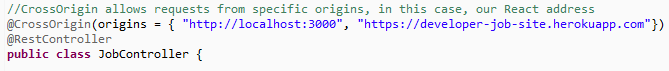
\includegraphics[scale=0.62]{Images/heroku1.png} 
    \label{heroku1_label}
    \caption{Permitting Cross Origin Requests}
\end{figure}

\subsubsection{2. Host my MongoDB Database on Atlas}
\paragraph{This was a relatively simple step and has mostly been covered already in the previous section on Atlas. I had to have my database in the cloud so it would be available to my API from anywhere at all times.}
\subsubsection{3. Deploy my React App}
\paragraph{I created another Heroku application for the front end. This is the address that the user uses. As stated above, I had to add the front ends Heroku address to the Spring Boot controller classes in order to allow cross origin requests to the API (Figure ~\ref{heroku1_label}). Once I did this the application was fully deployed. }

\section{React}
\paragraph{React (ReactJs) is a Javascript library for building user interfaces. React can be used as a base in the development of single-page or mobile applications. However, React is only concerned with rendering data to the Document Object Model (DOM), and so creating React applications usually requires the use of additional libraries for state management and routing \cite{React:wiki}. React Router is one such library I relied heavily upon for this application.}
\paragraph{React uses a tool called 'Babel' to convert ES6 into a backwards compatible version of JavaScript that can be run by older JavaScript engines \cite{Babel}. ES6 is a more modern version of Javascript that brings useful features to a project such as the use of the 'let' and 'const' keywords, the spread operator or even arrow functions all of which are present in my application.}
\subsection{Core Features}
\paragraph{Its most notable core feature, is the use of components and props. Components can be rendered to a particular element in the DOM using the React DOM library. When rendering a component, one can pass in values that are known as "props" \cite{React:components}. There are two types of components, 'functional components' and 'class components'. They differ in the fact that class components can hold 'state' values and can pass props to children (Figure ~\ref{react1_label}). Components are extremely useful as you can reuse them as many times as you need. They essentially return a section of the user interface. A well written 'Reactful' application would have lots of components each fulfilling its own purpose and nothing else. This makes an application maintainable.}
\begin{figure}[h]
    \centering
    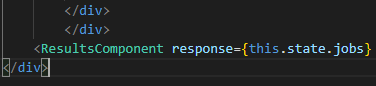
\includegraphics[scale=0.8]{Images/react1.png} 
    \label{react1_label}
    \caption{Passing a state value to 'ResultsComponent' as a prop called 'response'}
\end{figure}
\paragraph{Another notable features of React would be its use of 'Javascript-XML' (JSX). React uses JSX in place of HTML, it converts HTML tags into react elements. It is not required to use JSX in React although it is highly encouraged as it makes developing much easier. As demonstrated in (Figure ~\ref{react2_label}) the first line of code uses JSX, it lets us write HTML directly within a Javascript statement. Whereas in the second line, without the use of JSX, we must call the 'createElement' method and specify the tag. It's much easier to use JSX.}
\begin{figure}[ht]
    \centering
    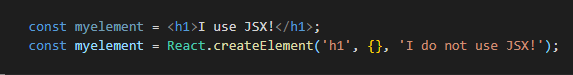
\includegraphics[scale=0.7]{Images/react2.png} 
    \label{react2_label}
    \caption{The same output, one with JSX and one without}
\end{figure}
\subsection{Creating React Application}
\paragraph{Like I did for creating my Spring Boot application, I made use of a very popular tool to help me speed up or 'bootstrap' the process of getting a React application off the ground. 'Create-React-App' is an official environment creator provided by the creators of React (Facebook) to help developers get set up to code within minutes. This powerful tool gets an application setup with the right set of dependencies such as babel, react-dom and ES6 without the developer ever having to worry.}
\paragraph{To use 'Create-React-App' one must have Node and Node-Package-Manager (NPM) installed. Then they simply run 'npx create-react-app <application name>' and let their environment get setup.}
\paragraph{Lastly, to run the react application in development mode we use the command 'npm start'. This runs the application on 'localhost:3000'.}

\section{JSON Web Tokens}
\paragraph{As mentioned earlier, my application would need some form of authentication. For this, I used JSON Web Tokens (JWT). JWT is an open standard that defines a compact and self-contained way for securely transmitting information between parties as a JSON object. This information can be verified and trusted because it is digitally signed. JWTs can be signed using a secret or a public/private key pair \cite{JWT}, in regards to my application - a secret.}
\begin{figure}[ht]
    \centering
    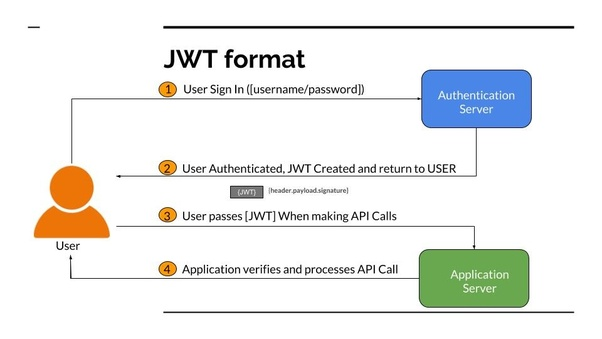
\includegraphics[scale=0.4]{Images/jwt1.jpeg} 
    \label{jwt1_label}
    \caption{JWT process}
\end{figure}
\paragraph{Specifically, JWT was used for authenticating and authorizing requests to and from my React application to my RESTful API. Below is a broad example of the steps that take place in my application when a user logs in:}
\begin{itemize}
    \item The user sends a POST request to the '/authenticate' endpoint with a username and password. 
    \item The credentials are verified on the back end and a JWT is returned using a secret.
    \item The JWT and username are committed to the browser's session storage (not the password as it is sensitive data), this allows for verification on future requests.
    \item All subsequent API calls contain this JWT in their  authorization header using 'axios interceptors'.
    \item Application verifies whether or not the user is logged in (via session storage) and the JWT and then processes the request.
\end{itemize} 

% Not sure whether to go into detail here on how JWT is implemented in my project. Would take up at least two more pages with all the screenshots that would be neccessary

%RESTful api?
\section{Secondary Technologies}
\paragraph{In this section I'll briefly analyze some of the secondary technologies and programs I used throughout the project that I found useful in development and think would be worthwhile mentioning.}
\subsection{Postman}
\paragraph{Postman is a fantastic collaboration platform for API development. It makes it easy for developers to test and document their API as well as save requests in collections and share them with peers. Users can send basic HTTP requests or configure complex requests detailing a range of different authentication types, as well as read their responses. It also lets you send and receive data in a number of different formats such as XML, JSON or even HTML.}
\paragraph{Postman is much more pleasant than using a browser and displays data really well. Below (Figure ~\ref{postman_label}) I have outlined some of the main components of my Postman environment:}
\begin{enumerate}
    \item This area displays  the collections I created. Initially I just had one collection - 'Job API'. This grouped requests connecting to my locally hosted API, however after deploying the API to Heroku, I created a second collection for requests to that. Each collection groups requests into the 4 main HTTP request methods.
    \item This is where you enter the address and endpoint of the API you wish to connect to as well as the HTTP request method type.
    \item This is the request section. As shown below, I am making a POST request to the '/authenticate' endpoint, I'm passing it a username and password. If I was making a request to a different endpoint, I would include a JWT token in the 'Authorization' tab.
    \item This is the response section. As we can see, the server sent me back a JWT token. This area also shows the status of the request, in this case, '200 OK'. 
\end{enumerate}
\begin{figure}[ht]
    \centering
    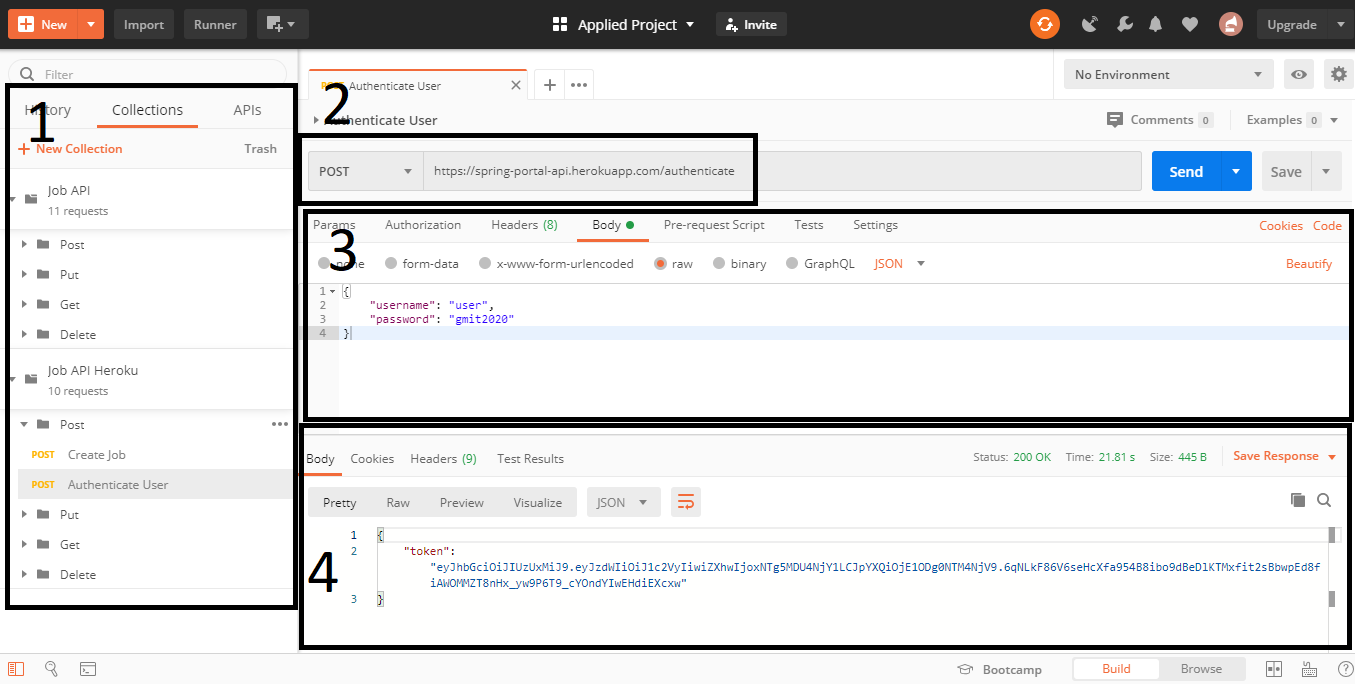
\includegraphics[scale=0.3]{Images/postman.png} 
    \label{postman_label}
    \caption{Postman home screen}
\end{figure}

\subsection{GitHub}
\paragraph{As touched on in the Methodology chapter, GitHub was used throughout development to provide a back-up of my work and to document consistent progress over the seven or eight months I have been planning and developing the application. It's also very useful for version control and makes it easy to revert any changes to a project if a mistake is made via the commit history.}
\paragraph{As I had mentioned, I regret not using more of GitHub's features to their fullest such as the Wiki or the Issues tracker. I did make some entries to the 'Issues' tracker late on in the project when I realised it would've been beneficial (Figure ~\ref{postman_label}). I documented my thoughts and progress mostly in Trello and a simple Word document but would've made better use of these features given a second run at the project.}
\begin{figure}[h]
    \centering
    \begin{minipage}{0.5\textwidth}
        \centering
        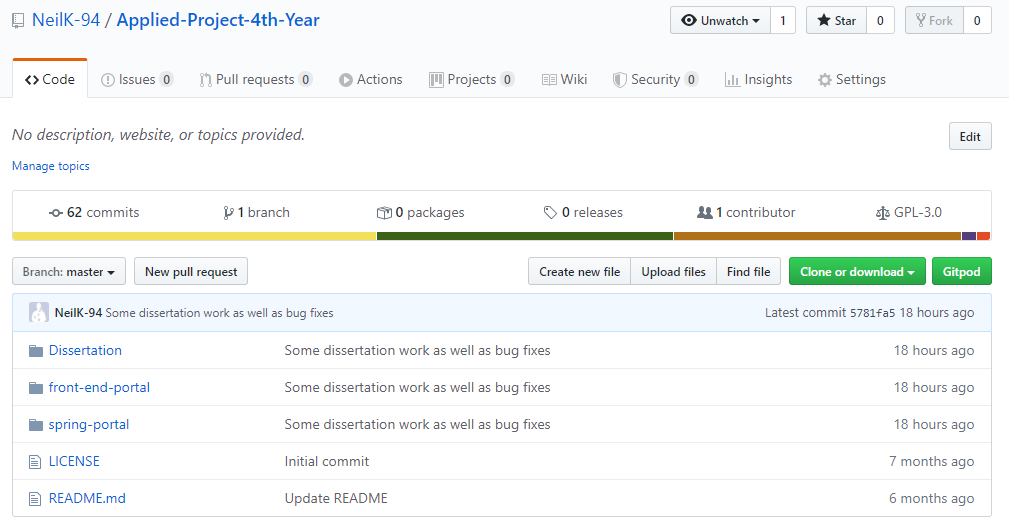
\includegraphics[scale=0.25]{Images/github1.png} 
        \label{git1_label}
        \caption{GitHub repository}
    \end{minipage}\hfill
    \begin{minipage}{0.5\textwidth}
        \centering
        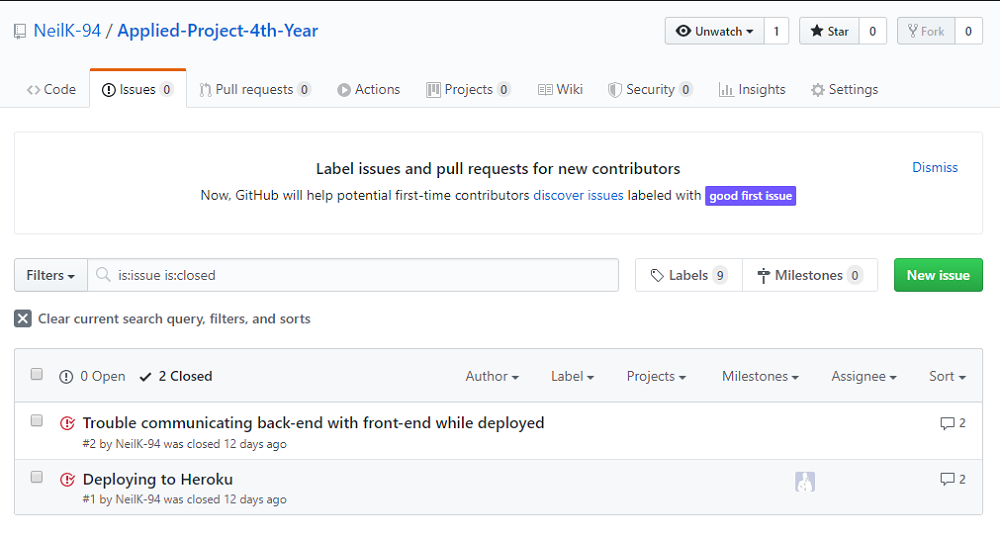
\includegraphics[scale=0.25]{Images/github2.png}
        \label{git2_label}
        \caption{GitHub issues tracker}
    \end{minipage}
\end{figure}

\subsection{React Frameworks}
\subsubsection{Many different frameworks were used alongside the React library to develop the front end application, some of the most notable are the following:}

\subsubsection{1. Bootstrap}
\paragraph{Bootstrap is an invaluable CSS framework which helps style web pages. I used it throughout my application and is used to style almost every component. I initially imported the Bootstrap CSS via the site 'UNPKG'. This is a useful content delivery site for everything on NPM. I simply added the URL to a 'bootstrap.css' file and then imported it into my app (Figure ~\ref{boot_label}). Later on in development I added it via NPM also for easier use of features such as forms.}
\begin{figure}[h]
    \centering
    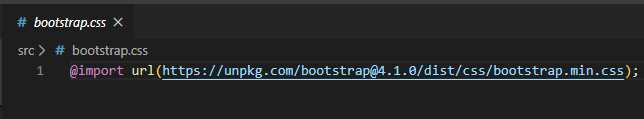
\includegraphics[scale=0.4]{Images/bootstrap1.png} 
    \label{boot_label}
    \caption{Bootstrap CSS file}
\end{figure}

\subsubsection{2. Axios}
\paragraph{Axios is a promise based HTTP client used to perform HTTP requests on API's. This framework was used for all requests coming and going from my front-end application.}
\begin{figure}[h]
    \centering
    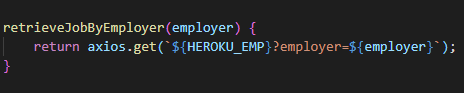
\includegraphics[scale=0.5]{Images/axios.png} 
    \label{axios_label}
    \caption{An Axios request}
\end{figure}

\subsubsection{3. React Router}
\paragraph{The React Router framework handles all the routing between components in my application. React Router is a widely used framework for React and can be found in most React applications. I used this framework extensively in my 'UserApp' component which acts as the central hub of my application. From here I control which web-pages are shown to the user(Figure ~\ref{router_label}), it is also used for authenticating all routes.}
\begin{figure}[h]
    \centering
    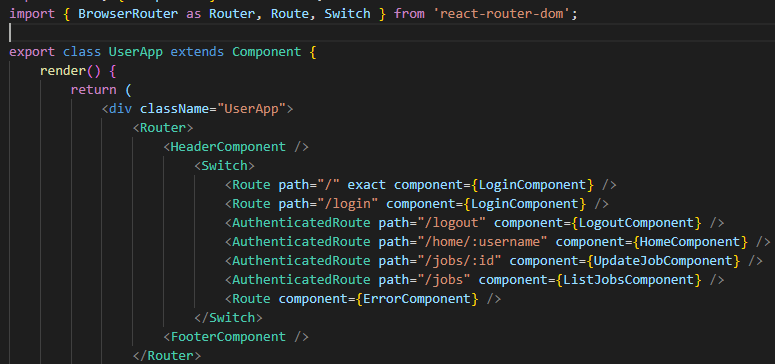
\includegraphics[scale=0.35]{Images/router.png} 
    \label{router_label}
    \caption{Main component using Router}
\end{figure}
\chapter{System Design}
\section{Architecture}

\begin{figure}[ht]
    \centering
    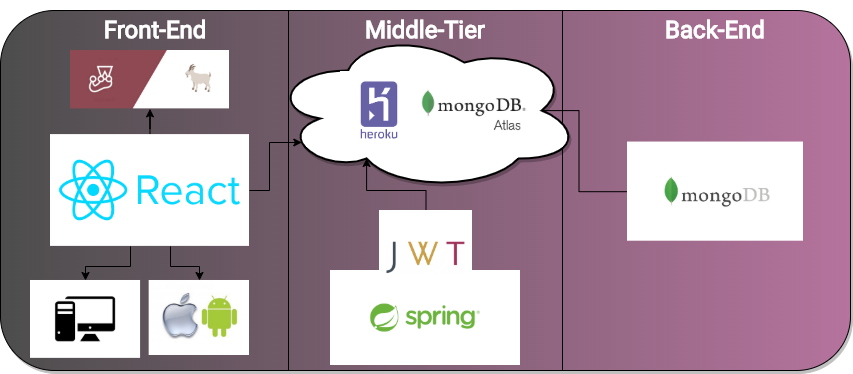
\includegraphics[scale=0.35]{Images/Project Architecture.png} 
    \label{proj_label}
    \caption{Project architecture diagram}
\end{figure}

The architecture (Figure ~\ref{proj_label}) of this project is comprised of three different tiers.
\begin{enumerate}
    \item The \textbf{Front-End} consists of the React application and of course all of the frameworks that go with it.
    \item The \textbf{Middle-tier} consists of my Spring Boot server which configures the REST API endpoints as well as the JWT API. These API's are of course, also hosted on Heroku and are in use by the front-end application to make requests.
    \item Lastly the \textbf{Back-End} which acts as a data tier includes a MongoDB database which stores all of the job details. I deployed the database on MongoDB Atlas to ensure the data is always available.
\end{enumerate}
In the following sections I will detail the design for each tier and explain why I made the decisions I did.

\section{Front End}
As this section contains the user interface, the only part of the application that the end user will actually see, I will go into extensive detail on it and provide many screenshots of each page and feature as well as provide some code snippets on how each feature was implemented.

\subsection{Login Page}
The login page (Figure ~\ref{login_label}) is the first page the user sees when they use my application. They cannot progress to any other pages in my application as all routes are authenticated. It consists of two text-boxes for entering user credentials, as well as a Bootstrap button for beginning the login sequence. If a user enters incorrect credentials they are alerted via a 'Bootstrap alert'. Further down the page there is a 'jumbotron' for styling purposes.

\begin{figure}[ht]
    \centering
    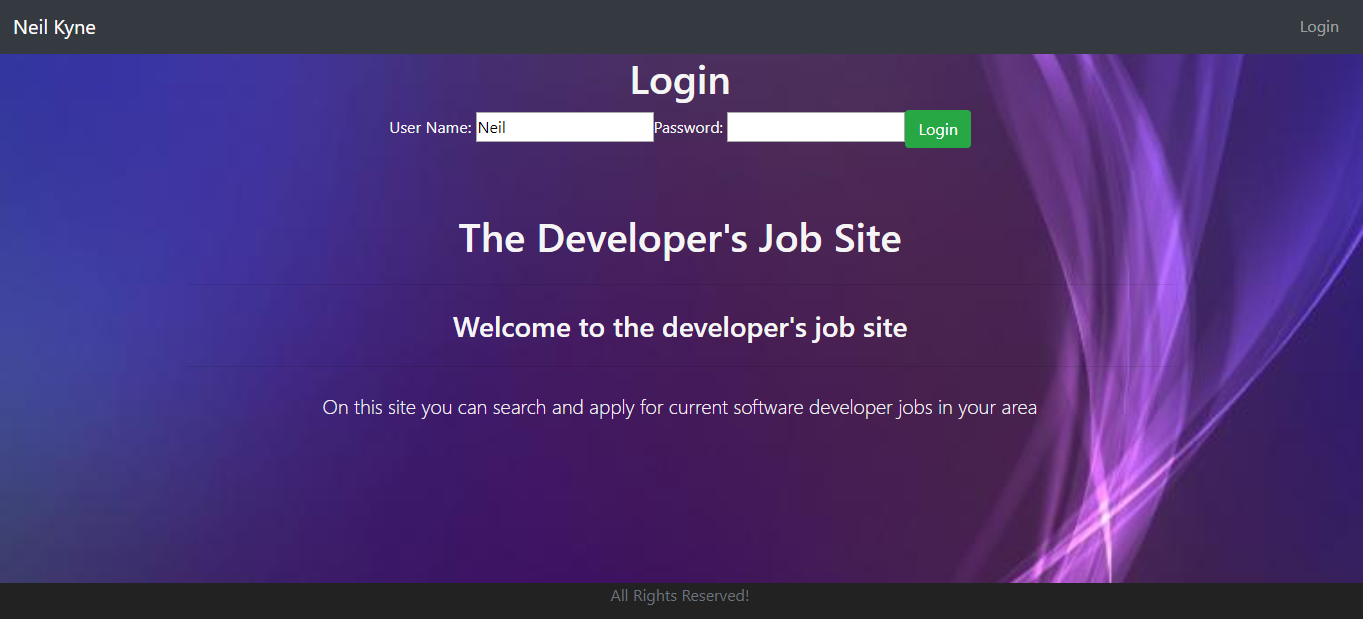
\includegraphics[scale=0.3]{Images/login.png} 
    \label{login_label}
    \caption{Login page}
\end{figure}

\subsection{Header \& Footer}
There is a navigation bar (Figure ~\ref{header_label}) at the top of every page in my application. This is useful for moving between pages and navigating the site. All routes in my application are authenticated meaning they cannot be accessed unless the user is logged in. Beginning from the left, it is comprised of;

\begin{figure}[ht]
    \centering
    
\includegraphics[scale=0.35]{Images/header.png} 
    \label{header_label}
    \caption{My 'navbar' at the top of every page}
\end{figure}
\begin{itemize}
    \item 'Neil Kyne' - This is a clickable link which simply takes the user to my GitHub profile.
    \item 'Home' - This brings the user to the home page.
    \item 'Jobs' - This brings the user to the full list of jobs.
    \item 'Logout' - This signs a user out and returns them to the login page.
\end{itemize}
Finally, just like the header, there is a footer at the bottom of every web-page. This just contains a generic 'All Rights Reserved' statement.

\subsection{Home Page}
The home page (Figure ~\ref{home_label}) is the core of the front-end application. It consists of four components:

\begin{figure}[ht]
    \centering
    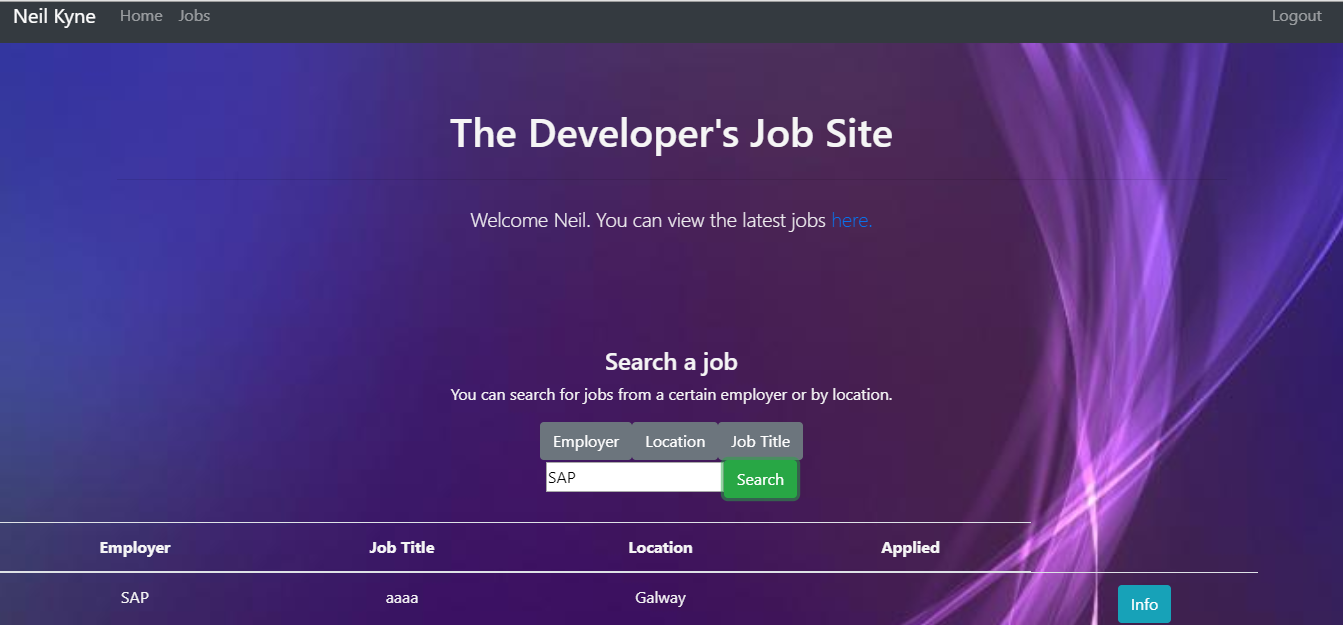
\includegraphics[scale=0.3]{Images/home.png} 
    \label{home_label}
    \caption{Home page}
\end{figure}

\subsubsection{1. Home Component}
This component simply acts as a greeting to the user. It comprises of a 'jumbotron' containing a welcome message for the user as well as a link to the full list of jobs.

\subsubsection{2. Search Component}
This component handles dynamic searching of jobs by their employer, location or job title.

\subsubsection{3. Results Component}
Here the results from the 'SearchComponent' are passed in as props to be displayed in a regular HTML table. Each row in the table has a 'View' button which opens up a Bootstrap 'Modal'.

\subsubsection{Apply Component}
This component (Figure ~\ref{apply_label}) is a 'modal' that displays more details about the job as well as gives an option to the user to apply for the job. If the user applies for that job they are notified via a Bootstrap alert and a marker is left beside the job in the table.

\begin{figure}[ht]
    \centering
    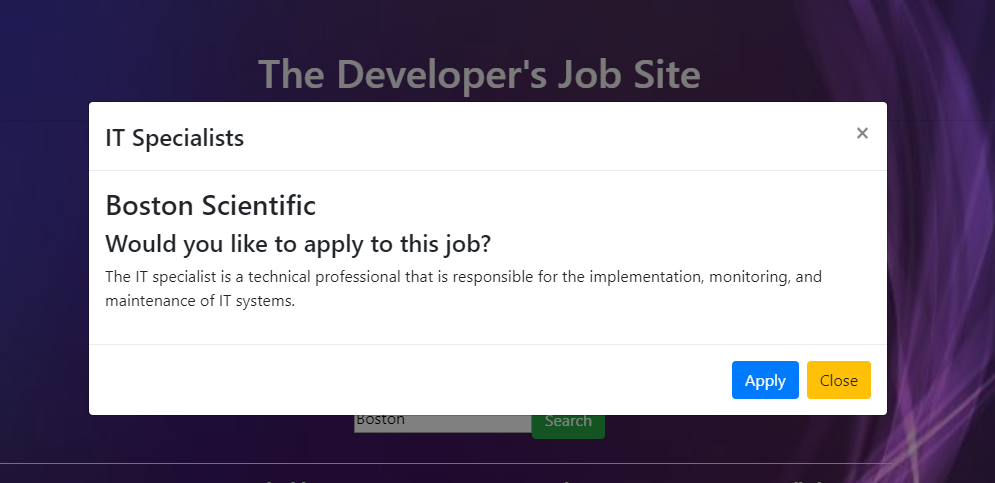
\includegraphics[scale=0.4]{Images/apply.png} 
    \label{apply_label}
    \caption{Apply modal}
\end{figure}

\subsection{Jobs Page}
This page (Figure ~\ref{jobs_label}) contains a 'Add' button which brings the user to the 'UpdateJobComponent'. The page also contains a table listing all the jobs in the database as well as two buttons in every row;

\begin{itemize}
    \item The \textbf{Delete button} removes a job listing from the database and refreshes the page.
    \item The \textbf{Update button} brings the user to the update job component.
\end{itemize}
\begin{figure}[ht]
    \centering
    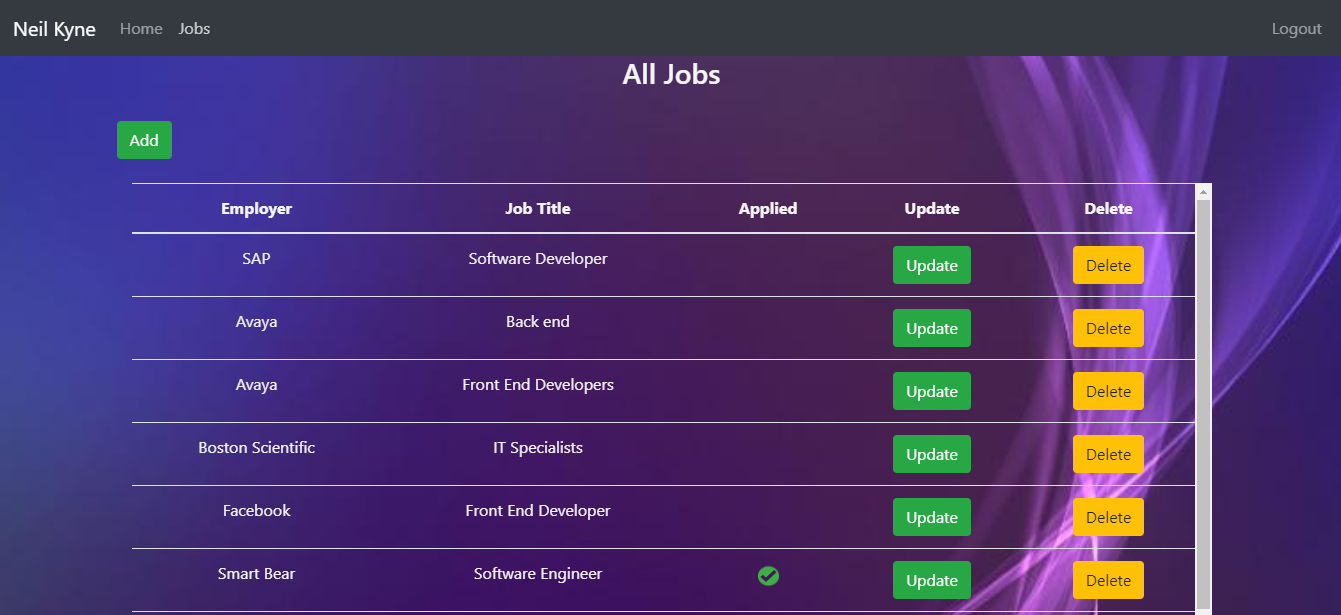
\includegraphics[scale=0.3]{Images/jobs.png} 
    \label{jobs_label}
    \caption{Jobs page}
\end{figure}

\subsection{Update/Create Job Page}
This page (Figure ~\ref{update_label}) acts as a two in one. If the user clicks on the update button in the 'ListJobsComponent' then the job details are passed in as props to this child component and the user can edit them. However if the user clicks on the add button in the previous component it will display an empty form for the user to fill in job details.

The form containing the job details is a React framework called 'Formik'. This is useful package that simplifies handling user data in React.

Lastly, the page has two buttons;
\begin{itemize}
    \item The \textbf{Save button} validates the form details, in my case it checks minimum character lengths in some of the text boxes. If they do not pass it displays a Bootstrap alert prompting the user to amend their mistake. If they pass validation it returns the user to the Jobs Page.
    \item The \textbf{Back button} returns the user to the previous page and discards any changes to the job.
\end{itemize}
\begin{figure}[ht]
    \centering
    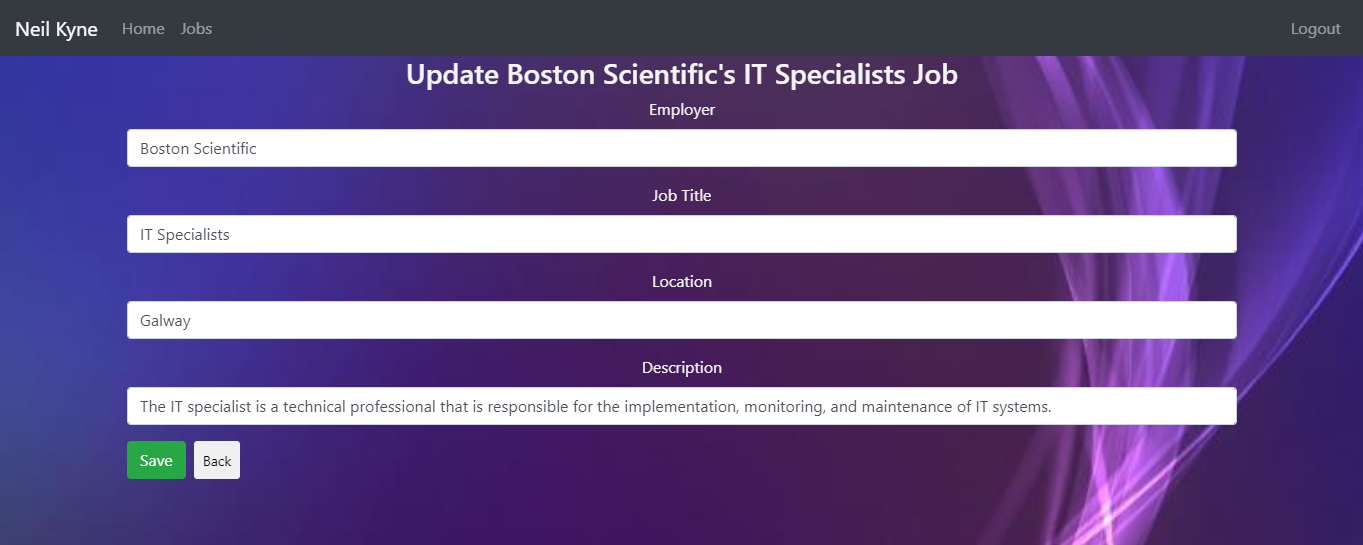
\includegraphics[scale=0.3]{Images/update.png} 
    \label{update_label}
    \caption{Update page}
\end{figure}

\section{Middle Tier}
This section consists of a lot of the logic and actual computation in my application. The most important part of this tier is of course the REST API. This is what the front-end communicates with to manipulate or remove data. This tier also contains a JWT API which allows users to request new tokens and prove authentication. Both of these API's are hosted on Heroku.

\subsection{Spring Boot Project Structure}
The REST API hosted on Heroku was built using Spring Boot. In this section I will summarize my project setup (Figure ~\ref{setup_label}) and design for building the API.

\begin{figure}[ht]
    \centering
    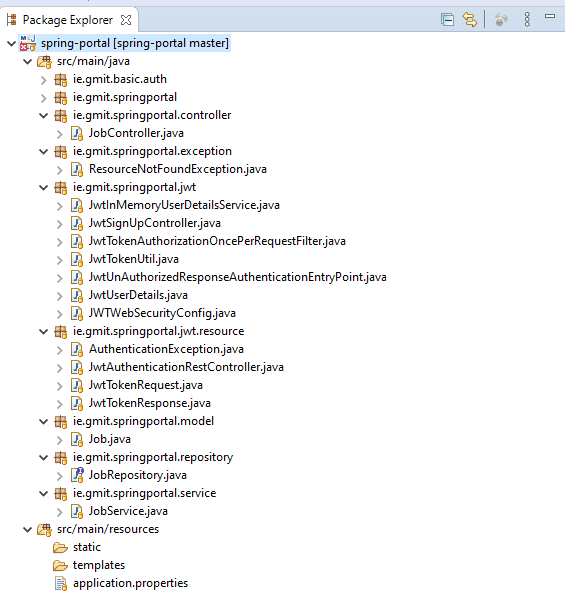
\includegraphics[scale=0.7]{Images/setup.png} 
    \label{setup_label}
    \caption{Project structure}
\end{figure}
%Might want to go into more detail on these..
\paragraph{My Boot project consists of four main packages;}
\begin{figure}[ht]
    \centering
    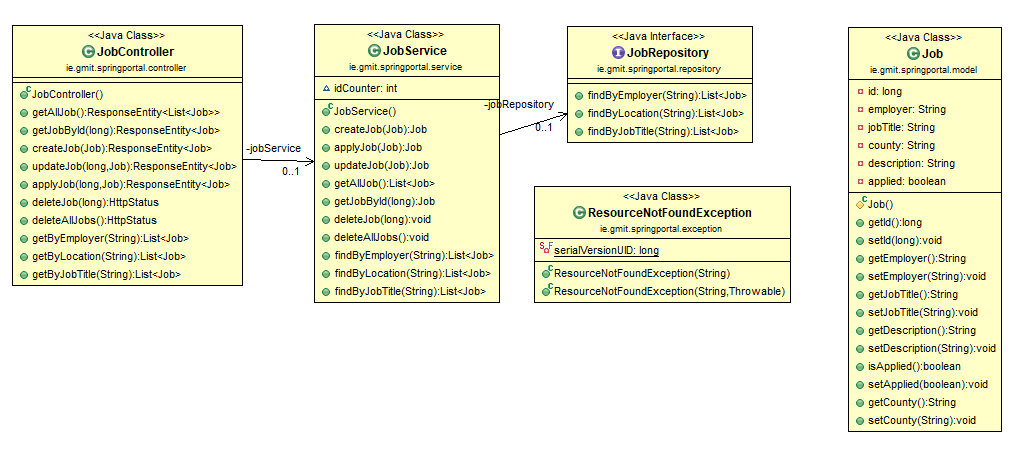
\includegraphics[scale=0.4]{Images/API UML.png} 
    \label{api_label}
    \caption{UML diagram of my API}
\end{figure}
\begin{itemize}
    \item The \textbf{Model} package describes the model that we want to work with, in this case a job. This is what is persisted to the MongoDB database and what is displayed at our front-end.
    \item The \textbf{Repository} package configures the MongoDB repository. The 'JobRepository' is used for accessing data from the database. It automatically implements all the basic CRUD operations one might want to perform on a database, I also added three custom methods for searching (Figure ~\ref{repo_label}). Spring Boot tries to auto-configure most of the stuff for you based on the dependencies that you have added in the pom.xml file.
    Since I added a 'spring-boot-starter-data-mongodb' dependency, Spring Boot automatically tries to build a connection with MongoDB by reading the database configuration from the 'application.properties' file.
    \begin{figure}[h]
    \centering
    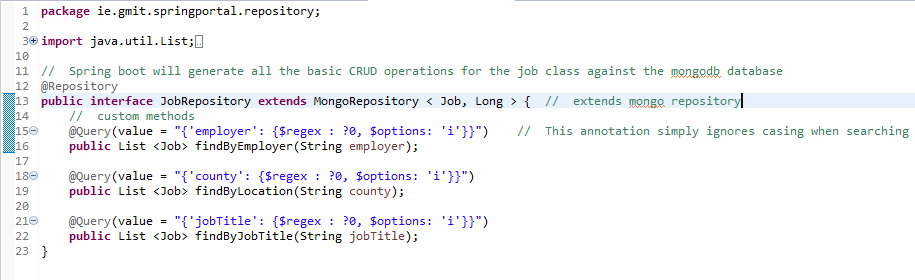
\includegraphics[scale=0.5]{Images/repo.png} 
    \label{repo_label}
    \caption{Mongo repository}
    \end{figure}
    \item The \textbf{Service} package describes the service layer. This package contains a lot of the business logic. The 'JobService' class connects with the 'JobRepository' class to perform CRUD operations on the database.
    \item Finally the \textbf{Controller} package contains the 'JobController' class. This is the API which will be exposed to the front-end users.
\end{itemize}


Aside from the listed packages there are;
\begin{itemize}
    \item A \textbf{Basic Authentication} package which is no longer in use as I now use JWT authentication.
    \item An \textbf{Exception} package for handling exceptions or errors with requests to the API.
    \item Two \textbf{JWT} packages.
        \begin{itemize}
            \item The resource package contains the resources related to the REST API and most importantly the 'JWTAuthenticationRestController'. This is the API we send requests to to receive JWT tokens.
            \item The JWT package contains all of the actual logic for creating the JWT token and the user details required to do so.
        \end{itemize}
        \begin{figure}[ht]
        \centering
        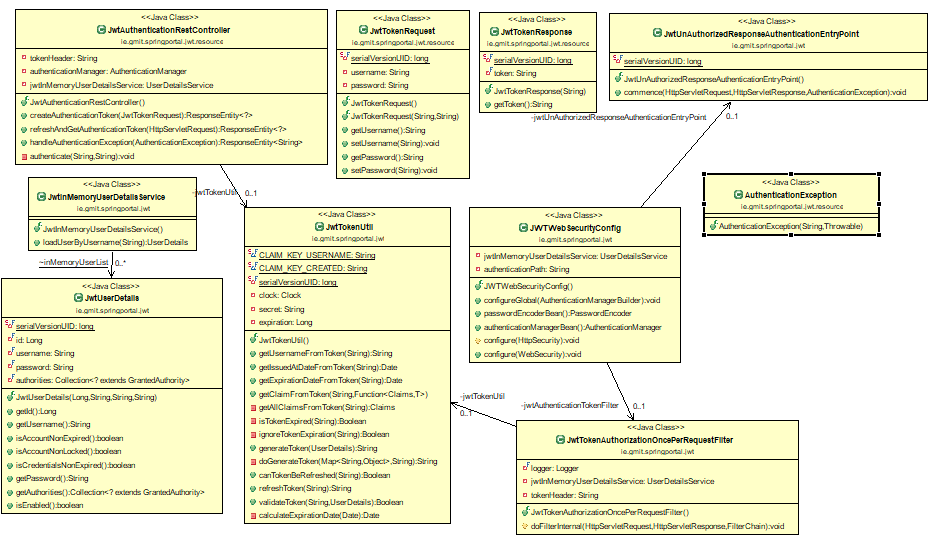
\includegraphics[scale=0.4]{Images/JWT UML.png} 
        \label{jwtuml_label}
        \caption{UML diagram for JWT packages}
        \end{figure}
        \item The \textbf{pom.xml} file contains project information and configuration information for maven to build the project such as dependencies, build directory and source directories. Maven reads the pom.xml file, then executes the goal \cite{POM}. Here (Figure ~\ref{pom_label}) I specified many dependencies to aid in building the API.
        \item Lastly, the \textbf{application.properties} file is used to keep project properties in a single file to run the application in a different environment.
\end{itemize}
\begin{figure}[ht]
    \centering
    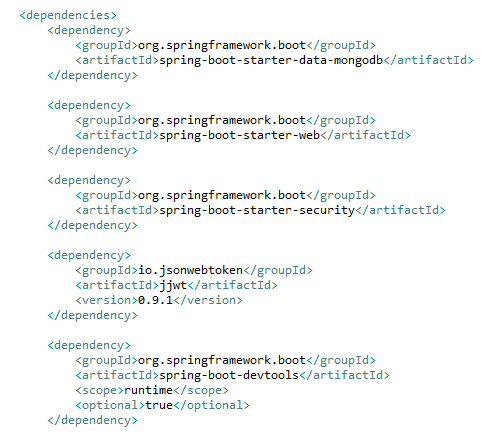
\includegraphics[scale=0.6]{Images/pom.png} 
    \label{pom_label}
    \caption{pom.xml file declaring dependencies}
\end{figure}

\subsection{Heroku}
In order for the React application to be able to access the API's online they would have to be hosted online. For this I used Heroku. To create an empty Heroku application via the Heroku Command Line Interface (CLI) I ran:

\begin{verbatim}
heroku create spring-portal-api
\end{verbatim}
To deploy the REST API to Heroku I first initialized a Git repository in my 'spring-portal' directory.

\begin{verbatim}
git init
\end{verbatim}
I then update the index using the current content found in the working tree, to prepare the content staged for the next commit.

\begin{verbatim}
git add .
\end{verbatim}
This stores the current content of the index in a new commit along with a message from the user describing the changes.

\begin{verbatim}
git commit -m "Added API to Heroku"
\end{verbatim}
Finally, to push to the new Heroku repository you use:

\begin{verbatim}
git push heroku master
\end{verbatim}

\section{Back-End}
The back-end tier stores all of my job data. I deployed my database online using MongoDB Atlas. This makes it available at all times to the API.

\subsection{MongoDB Atlas}
There were a number of steps required to deploy my database on Atlas.

\begin{enumerate}
    \item Create a MongoDB Atlas account.
    \item Create a free tier cluster by clicking "Build a new cluster". From here choose a cloud provider and region. Finally Choose the free tier cluster option, selecting the M0 sandbox (free tier) and name your cluster.
    \begin{itemize}
        \item Atlas Free Tier clusters provide a small-scale development environment to host your data. Free Tier clusters never expire, and provide access to a subset of Atlas features and functionality \cite{Atlas}.
    \end{itemize}
    \item Next, when the cluster is created, click 'Connect'. Here we white-list our IP address. Secondly, add yourself as a database user admin to allow for full access.
    \item Now we are ready to connect the cluster to the Spring Boot project. Click connect, configure the project settings and copy the string (Figure ~\ref{atlas1_label}).
    \item Head over to the 'application.properties' file and paste in the string, replacing the blank username and password with your own.
\end{enumerate}

\begin{figure}[h]
    \centering
    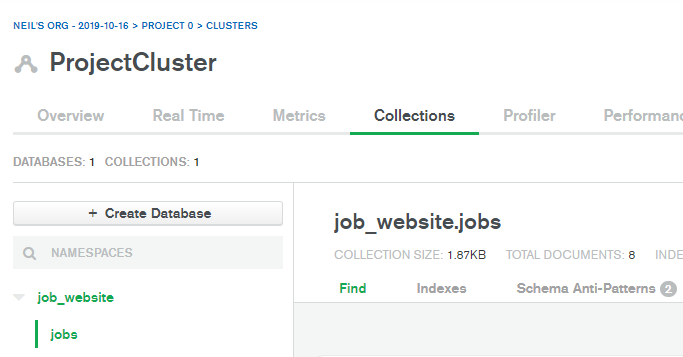
\includegraphics[scale=0.37]{Images/atlas2.png}
    \label{atlas2_label}
    \caption{Database with its 'jobs' collection}
\end{figure}
\begin{figure}[ht]
    \centering
    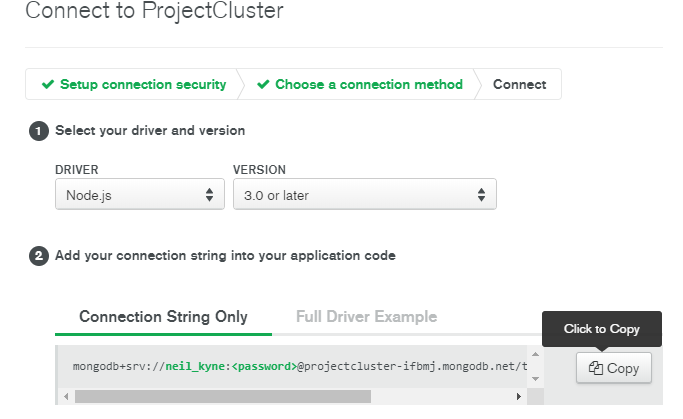
\includegraphics[scale=0.5]{Images/atlas.png} 
    \label{atlas1_label}
    \caption{Application connection string}
\end{figure}

It may have been noticed I never specified a name for the database or a name for the collection anywhere on MongoDB Atlas. All of this is configured in my Spring Boot application. I specify these details using the Spring data annotations provided for use with MongoDB. I also specify a few other settings for the 'Job' documents using these annotations (Figure ~\ref{atlas3_label}) such as the \textbf{@Id} of the document which is the identifier for every mongo document, as well as more basic annotations such as \textbf{@NotBlank} which forbids empty values and \textbf{@Size} which allows a user to set a max input size.

I define the collection name in the database above the class declaration with \textbf{@Document(collection = "jobs")}. Finally the database name is declared in the 'application.properties' file with \newline \textbf{spring.data.mongodb.database=job\_website}.

\begin{figure}[ht]
    \centering
    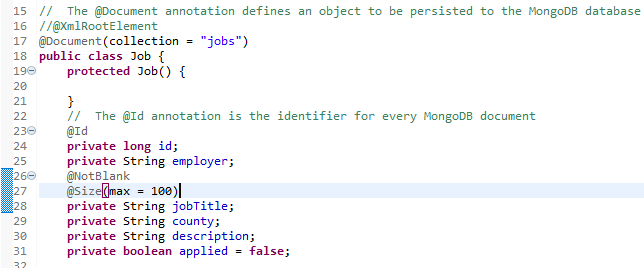
\includegraphics[scale=0.5]{Images/atlas3.png}
    \label{atlas3_label}
    \caption{Job model outlining some mongo configurations using Spring-Mongo annotations.}
\end{figure}


\chapter{System Evaluation}
In this section I will look to give a critical analysis of my application, I will compare the objectives I set out at the beginning of the project with what I actually managed to achieve. I will also call attention to the shortcomings in the application as well as areas I feel could be improved upon.


\section{Initial Objectives}
In my introduction I set out a number of objectives I wanted to accomplish with this project. Here I will examine each one and determine whether or not I feel I accomplished them sufficiently.

\subsubsection{Objective 1}
My first objective was to build an application 'with a number of moving parts'. This essentially means I wanted it to be a full stack application. A full stack developer is a person who can develop both client and server software \cite{FullStack}. I really wanted to do this because, as I mentioned earlier on in the document, I felt it would be important to experience what it's like to build a real, genuine web application from top to bottom. I feel I achieved this objective as my application covers every 'stack'.

\subsubsection{Objective 2}
My second objective was to become 'very familiar' with React. Again I do feel that I have accomplished this objective. I would say technology wise, the project consists of about 60\% React/Javascript code while the rest is made up of Java and a few others. I had wanted to become familiar with React as it is an ever increasing language in terms of popularity and I wish to focus on web development once I graduate. I'm far from an expert with React having finished the application but I will say I feel I developed genuine knowledge on the technology that I can use as a base to build on in the future.

\subsubsection{Objective 3}
My third objective was for the application to have authentication. I decided ideally, the application would use JWT but failing that would use basic authentication. I initially implemented basic authentication and from there managed to upgrade the project authentication to JWT.

\subsubsection{Objective 4}
My fourth objective was for the user to be able to perform the basic CRUD functions on the API. This was one of the first things I achieved and added to by implementing custom searches.

\subsubsection{Objective 5}
Finally, my fifth and final objective was to get the entire application deployed and running on Heroku. This was the last objective I managed and had a reasonable degree of difficulty in achieving. It involved deploying the back-end API and the front-end application as two separate Heroku applications. It was also required for my database to be deployed on MongoDB Atlas to ensure the data was available at all times to the API.

\section{Limitations \& Improvements}
Sadly, my project has its limitations. Due to a mix of adverse time management and to a degree, lack of knowledge of the technologies used, my application has many areas I feel could be improved on. Hindsight is a wonderful thing, given what I know know there are plenty of things I would do differently if given the chance to go back and start again.

\subsection{Sign Up Functionality}
One of my biggest regrets with the project is that I never got around to implementing a sign up option. This wouldn't have been too difficult to do but in the end I ran out of time. When I first implemented JWT I hard-coded two user profiles into the user details service. I kept putting off adding the ability to create new user profiles in favor of more pressing work and in the end never implemented it at all.

To do this, I would have needed to create new 'Controller', 'Model' and 'Service' classes for user sign-ups around the 'JWTInMemoryUserDetailsService'. I would then have needed to simply update the 'JWTWebSecurityConfig' class to allow calls to a '/signup' endpoint without authentication.

Once I had that working on the back-end I would have added a sign-up option to the login page which would use Axios to send a request to the '/signup' endpoint, passing in the new username and password. This would've been a nice addition to the login page as it is a bit bare without it.

\subsection{More Complex API}
With this application I knew I wanted to focus slightly more on the front-end than the back. As a result, I feel my REST API was a little neglected in terms of features. Looking back, I would definitely have liked to add more complex features to my API such as searching within specific constraints (like only searching for jobs in multiple different locations).

I feel the actual job details could've been extended upon and included contact details, salaries and experience requirements just to name a few.

\subsection{More Front-End Features}
Finally, I would've liked to have added more 'bells \& whistles' with the front-end of my application. There are many really interesting frameworks that can make React applications more user friendly and outside of purely functional frameworks such as Axios, I feel I only really used React Bootstrap to make the visual side of the application more appealing. I suppose using the knowledge gained from this project learning React, I will be more capable of adding such features to web applications in the future.

\subsection{Much More Testing}
Throughout development I kept telling myself I would get round to implementing detailed testing when the application was finished. This was rather naive of me as it is well known in modern software development that developers are expected to run their own tests as they go and not rely on testing teams. This was even covered in one of our modules and I majorly regret not heeding this advice.

\section{Testing}
I incorporated a small handful of test in my front-end application using Jest and React-Testing-Library. I mainly tested UI elements of the application and only on two components, the 'LoginComponent' and the 'SearchComponent'.

By default \textbf{Jest} expects to find files to test in a '\_\_test\_\_' folder (Figure ~\ref{test4_label}). These files must end with '.test.js'. Ideally if there were tests being done on every component in my application, it might be useful to group every component into their own sub folder along with their test file and perhaps their styling file. This would keep the project directory clean and tidy and is something I will look to do in future projects.

\begin{figure}[ht]
    \centering
    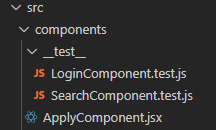
\includegraphics[scale=0.8]{Images/test4.png} 
    \label{test4_label}
    \caption{Jest required project layout}
\end{figure}

\subsubsection{LoginComponent Tests}
In the 'LoginComponent' I run three tests, the first two are contained in the first 'describe'. \textbf{Describe} is a function name, along with \textbf{it} in a lot of testing framework. It essentially groups together tests into suites.

The first test suite checks to see first, that the component renders correctly, and then to see that the login button renders correctly, with the correct content inside it(Login).

The second tests to ensure that the input box containing the placeholder text, 'Neil' updates on change. It passes the value 'test' into it using a \textbf{fireEvent}. fireEvents are useful for performing an action in a test. Finally, we use the \textbf{expect} function to tell our test what value to expect the searchInput value to be.

\begin{figure}[ht]
    \centering
    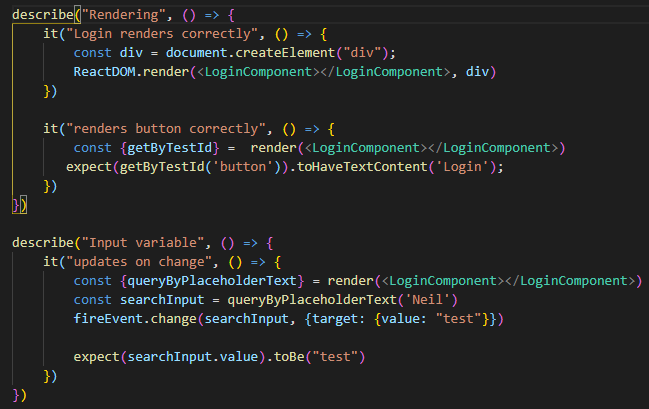
\includegraphics[scale=0.5]{Images/5.png} 
    \label{test5_label}
    \caption{LoginComponent tests}
\end{figure}
\begin{figure}[ht]
    \centering
    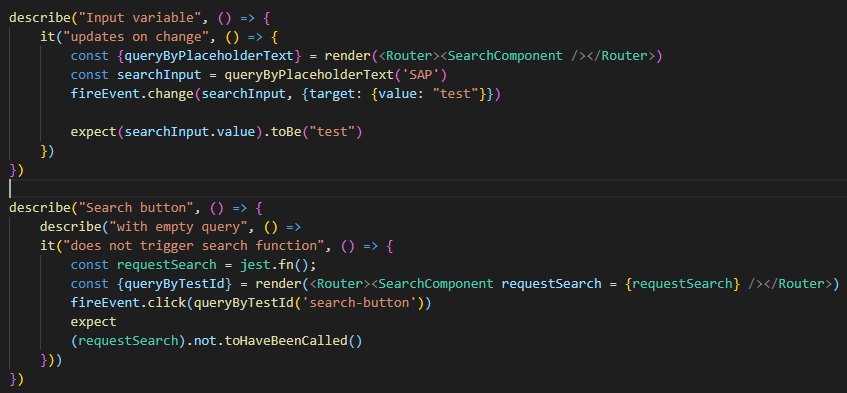
\includegraphics[scale=0.4]{Images/test3.png} 
    \label{test3_label}
    \caption{Some SearchComponent tests}
\end{figure}

\newpage
\subsubsection{SearchComponent}
In the 'SearchComponent' test file I perform three main tests as well as a test to check that the component renders correctly.

The first test, like in the 'LoginComponent' test file, checks to ensure that the 'textBox' value changes when we pass in a test value.

Next I check to ensure that the 'searchButton' when clicked without a query given, does not trigger a search. To do this I use a Jest Mock which is a function that essentially mimics the behaviour of an object. This is then passed in as a prop to the SearchComponent.

Finally, I reverse the previous test to check that when there is data given in a query, and the user clicks the 'searchButton' it would trigger a search.

\subsubsection{Running The Tests}
Running the tests is simple. As Jest comes pre-configured with 'create-react-app' you need only run:

\begin{verbatim}
    npm test
\end{verbatim}
\begin{figure}[ht]
    \centering
    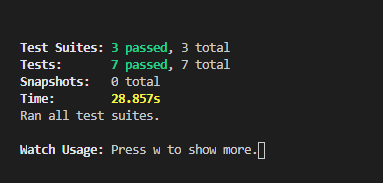
\includegraphics[scale=0.9]{Images/test2.png} 
    \label{test2_label}
    \caption{Test results}
\end{figure}
\chapter{Conclusion}
\section{Project Outcomes}
\paragraph{When I began this project I had a reasonably clear idea of what I wanted the project to be;}
\begin{itemize}
    \item A job site aimed specifically at software developers which hosted software development jobs.
    \item The user should be able to log in securely using a username and password.
    \item The user should be able to search for jobs by a number of different methods.
    \item The user should be able to post their own jobs and delete or update them.
    \item The front end website should be visually appealing with a handful of neat features.
    \item The API should be RESTful.
    \item The application should be hosted online and accessible at all times.
    \item The job data should be deployed on a cloud database.
    \item There should be tests verifying the integrity and solidity of my front-end application.
\end{itemize}
\paragraph{I feel I achieved most of the goals I had when I set out with this project. Of course, there is plenty of limitations and room for improvements, however I do feel that I have gained a lot from the project and if I was to go back and start it again, would still choose the technologies that I did.}
\paragraph{I created what I believe to be, a decently sized project for a one person group. I believe in covering the different parts of the stack I was exposed to a number of different technologies and thus gained valuable experience in full stack development. It was very important for me from the beginning that it was a full stack application and thankfully I achieved that. }
\subsection{My Findings}
\paragraph{I learned a number of things in undertaking this project and will review some below:}
\begin{itemize}
    \item React is a very enjoyable technology to use and I will certainly look to improve upon it further in the future.
    \item Undertaking a full stack application solidified my desire to work with web applications in the future.
    \item It is very important to adequately plan out a project of this scope and hold yourself to deadlines and targets.
    \item Testing should be done alongside development to ensure bugs are caught early and code is clean and reusable.
    \item Project management is a very important skill to have when working with multiple different projects. It is essential that you dedicate time every week to a project, even if other ones are more pressing. Even spending an hour or two a week on a project that isn't as pressing as another at the time, you ensure you retain key information and continue learning about the technology.
\end{itemize}
\section{Summary}
% Mention how it went, what you learned, what is it rewarding, challenges faced etc, scope big enough? 
\paragraph{In conclusion I must say that overall I have genuinely found the project to be very rewarding. It helped me to gain a decent grasp on a number of new technologies as well as forced me to learn how to manage a larger project than I'm used to doing over a large time-frame. I was forced to comprehensively research multiple technologies and find pros and cons to using each one. This project also demanded I set out a clear plan of action for what I wanted to achieve and within what time-frame.}
\paragraph{I think the main goals of this module were to learn how to manage a demanding project over a large period of time and to showcase the ability to set out and learn new technologies without being taught them by a lecturer in class. I do believe I have achieved both of these and had a lot of fun along the way. This project has confirmed for me what I want to do after college and I'm very glad I made the decisions I did. Naturally, not everything went perfectly as I would have liked but the shortcomings I faced have taught me a lot going forward.}
\chapter{Appendices}
\section{GitHub Repository}
\paragraph{https://github.com/NeilK-94/Applied-Project-4th-Year}

%----------------------------------------------------------------------------------------
\bibliographystyle{unsrt}
\bibliography{references.bib}
\end{document}